\hypertarget{md5__loc_8h}{
\section{md5/md5\_\-loc.h File Reference}
\label{md5__loc_8h}\index{md5/md5\_\-loc.h@{md5/md5\_\-loc.h}}
}
Diese Funktionen liefern die Moeglichkeit, einen MD5-Hash eines beliebigen String zu generieren. 



This graph shows which files directly or indirectly include this file:\nopagebreak
\begin{figure}[H]
\begin{center}
\leavevmode
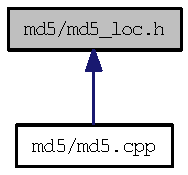
\includegraphics[width=63pt]{md5__loc_8h__dep__incl}
\end{center}
\end{figure}
\subsection*{Defines}
\begin{CompactItemize}
\item 
\#define \hyperlink{md5__loc_8h_edbcc427391a12db8072aa23472b2c18}{HEX\_\-STRING}~\char`\"{}0123456789abcdef\char`\"{}
\item 
\#define \hyperlink{md5__loc_8h_922a001b47a0d088e36929b15dafeee8}{BLOCK\_\-SIZE\_\-MASK}~(MD5\_\-BLOCK\_\-SIZE - 1)
\item 
\#define \hyperlink{md5__loc_8h_bc379298e18c4c5a44fbb37e0f5a36fa}{FF}(b, c, d)~(d $^\wedge$ (b \& (c $^\wedge$ d)))
\item 
\#define \hyperlink{md5__loc_8h_5b02b4f5acc69dd3dae769e317cafba8}{FG}(b, c, d)~FF(d, b, c)
\item 
\#define \hyperlink{md5__loc_8h_2755ce913ebfebd237cf80feb99a0a59}{FH}(b, c, d)~(b $^\wedge$ c $^\wedge$ d)
\item 
\#define \hyperlink{md5__loc_8h_c8cd4262e1565a47dfbbb66be56e3e6c}{FI}(b, c, d)~(c $^\wedge$ (b $|$ $\sim$d))
\item 
\#define \hyperlink{md5__loc_8h_cbfb625da1590a909133dace59d0fc59}{CYCLIC}(w, s)~((w $<$$<$ s) $|$ (w $>$$>$ (32 - s)))
\item 
\#define \hyperlink{md5__loc_8h_ea05e0e1ca3cc9eb2f4b248bf86a590b}{OP1}(a, b, c, d, b\_\-p, c\_\-p, s, T)
\item 
\#define \hyperlink{md5__loc_8h_943a15a4fa9e5f60a6b66a6fcce01bf5}{OP234}(FUNC, a, b, c, d, k, s, T)
\end{CompactItemize}


\subsection{Detailed Description}
Diese Funktionen liefern die Moeglichkeit, einen MD5-Hash eines beliebigen String zu generieren. 

\begin{Desc}
\item[Version:]1.7 \end{Desc}
\begin{Desc}
\item[Date:]05.03.2006 \end{Desc}
\begin{Desc}
\item[Author:]Gray Watson \end{Desc}


Definition in file \hyperlink{md5__loc_8h-source}{md5\_\-loc.h}.

\subsection{Define Documentation}
\hypertarget{md5__loc_8h_922a001b47a0d088e36929b15dafeee8}{
\index{md5\_\-loc.h@{md5\_\-loc.h}!BLOCK\_\-SIZE\_\-MASK@{BLOCK\_\-SIZE\_\-MASK}}
\index{BLOCK\_\-SIZE\_\-MASK@{BLOCK\_\-SIZE\_\-MASK}!md5_loc.h@{md5\_\-loc.h}}
\subsubsection[BLOCK\_\-SIZE\_\-MASK]{\setlength{\rightskip}{0pt plus 5cm}\#define BLOCK\_\-SIZE\_\-MASK~(MD5\_\-BLOCK\_\-SIZE - 1)}}
\label{md5__loc_8h_922a001b47a0d088e36929b15dafeee8}




Definition at line 48 of file md5\_\-loc.h.

Referenced by md5\_\-process().\hypertarget{md5__loc_8h_cbfb625da1590a909133dace59d0fc59}{
\index{md5\_\-loc.h@{md5\_\-loc.h}!CYCLIC@{CYCLIC}}
\index{CYCLIC@{CYCLIC}!md5_loc.h@{md5\_\-loc.h}}
\subsubsection[CYCLIC]{\setlength{\rightskip}{0pt plus 5cm}\#define CYCLIC(w, \/  s)~((w $<$$<$ s) $|$ (w $>$$>$ (32 - s)))}}
\label{md5__loc_8h_cbfb625da1590a909133dace59d0fc59}


It is unfortunate that C does not provide an operator for cyclic rotation. Hope the C compiler is smart enough. -- Modified to remove the w = at the front - Gray 2/97 

Definition at line 86 of file md5\_\-loc.h.\hypertarget{md5__loc_8h_bc379298e18c4c5a44fbb37e0f5a36fa}{
\index{md5\_\-loc.h@{md5\_\-loc.h}!FF@{FF}}
\index{FF@{FF}!md5_loc.h@{md5\_\-loc.h}}
\subsubsection[FF]{\setlength{\rightskip}{0pt plus 5cm}\#define FF(b, \/  c, \/  d)~(d $^\wedge$ (b \& (c $^\wedge$ d)))}}
\label{md5__loc_8h_bc379298e18c4c5a44fbb37e0f5a36fa}


Define my endian-ness. Could not do in a portable manner using the include files -- grumble.

These are the four functions used in the four steps of the MD5 algorithm and defined in the RFC 1321. The first function is a little bit optimized (as found in Colin Plumbs public domain implementation). 

Definition at line 76 of file md5\_\-loc.h.\hypertarget{md5__loc_8h_5b02b4f5acc69dd3dae769e317cafba8}{
\index{md5\_\-loc.h@{md5\_\-loc.h}!FG@{FG}}
\index{FG@{FG}!md5_loc.h@{md5\_\-loc.h}}
\subsubsection[FG]{\setlength{\rightskip}{0pt plus 5cm}\#define FG(b, \/  c, \/  d)~FF(d, b, c)}}
\label{md5__loc_8h_5b02b4f5acc69dd3dae769e317cafba8}




Definition at line 77 of file md5\_\-loc.h.\hypertarget{md5__loc_8h_2755ce913ebfebd237cf80feb99a0a59}{
\index{md5\_\-loc.h@{md5\_\-loc.h}!FH@{FH}}
\index{FH@{FH}!md5_loc.h@{md5\_\-loc.h}}
\subsubsection[FH]{\setlength{\rightskip}{0pt plus 5cm}\#define FH(b, \/  c, \/  d)~(b $^\wedge$ c $^\wedge$ d)}}
\label{md5__loc_8h_2755ce913ebfebd237cf80feb99a0a59}




Definition at line 78 of file md5\_\-loc.h.\hypertarget{md5__loc_8h_c8cd4262e1565a47dfbbb66be56e3e6c}{
\index{md5\_\-loc.h@{md5\_\-loc.h}!FI@{FI}}
\index{FI@{FI}!md5_loc.h@{md5\_\-loc.h}}
\subsubsection[FI]{\setlength{\rightskip}{0pt plus 5cm}\#define FI(b, \/  c, \/  d)~(c $^\wedge$ (b $|$ $\sim$d))}}
\label{md5__loc_8h_c8cd4262e1565a47dfbbb66be56e3e6c}




Definition at line 79 of file md5\_\-loc.h.\hypertarget{md5__loc_8h_edbcc427391a12db8072aa23472b2c18}{
\index{md5\_\-loc.h@{md5\_\-loc.h}!HEX\_\-STRING@{HEX\_\-STRING}}
\index{HEX\_\-STRING@{HEX\_\-STRING}!md5_loc.h@{md5\_\-loc.h}}
\subsubsection[HEX\_\-STRING]{\setlength{\rightskip}{0pt plus 5cm}\#define HEX\_\-STRING~\char`\"{}0123456789abcdef\char`\"{}}}
\label{md5__loc_8h_edbcc427391a12db8072aa23472b2c18}




Definition at line 47 of file md5\_\-loc.h.

Referenced by md5\_\-sig\_\-from\_\-string(), and md5\_\-sig\_\-to\_\-string().\hypertarget{md5__loc_8h_ea05e0e1ca3cc9eb2f4b248bf86a590b}{
\index{md5\_\-loc.h@{md5\_\-loc.h}!OP1@{OP1}}
\index{OP1@{OP1}!md5_loc.h@{md5\_\-loc.h}}
\subsubsection[OP1]{\setlength{\rightskip}{0pt plus 5cm}\#define OP1(a, \/  b, \/  c, \/  d, \/  b\_\-p, \/  c\_\-p, \/  s, \/  T)}}
\label{md5__loc_8h_ea05e0e1ca3cc9eb2f4b248bf86a590b}


\textbf{Value:}

\begin{Code}\begin{verbatim}do {                                                    \
       memcpy(c_p, b_p, sizeof(md5_uint32));                    \
       *c_p = SWAP(*c_p);                                       \
       a += FF (b, c, d) + *c_p + T;                            \
       a = CYCLIC (a, s);                                       \
       a += b;                                                  \
       b_p = (char *)b_p + sizeof(md5_uint32);                  \
       c_p++;                                                   \
    } while (0)
\end{verbatim}
\end{Code}
First Round: using the given function, the context and a constant the next context is computed. Because the algorithms processing unit is a 32-bit word and it is determined to work on words in little endian byte order we perhaps have to change the byte order before the computation. To reduce the work for the next steps we store the swapped words in the array CORRECT\_\-WORDS. -- Modified to fix the handling of unaligned buffer spaces - Gray 7/97 

Definition at line 97 of file md5\_\-loc.h.\hypertarget{md5__loc_8h_943a15a4fa9e5f60a6b66a6fcce01bf5}{
\index{md5\_\-loc.h@{md5\_\-loc.h}!OP234@{OP234}}
\index{OP234@{OP234}!md5_loc.h@{md5\_\-loc.h}}
\subsubsection[OP234]{\setlength{\rightskip}{0pt plus 5cm}\#define OP234(FUNC, \/  a, \/  b, \/  c, \/  d, \/  k, \/  s, \/  T)}}
\label{md5__loc_8h_943a15a4fa9e5f60a6b66a6fcce01bf5}


\textbf{Value:}

\begin{Code}\begin{verbatim}do {                                            \
      a += FUNC (b, c, d) + k + T;                      \
      a = CYCLIC (a, s);                                \
      a += b;                                           \
    } while (0)
\end{verbatim}
\end{Code}
Second to Fourth Round: we have the possibly swapped words in CORRECT\_\-WORDS. Redefine the macro to take an additional first argument specifying the function to use. 

Definition at line 113 of file md5\_\-loc.h.